\chapter{Testautomatisierung}
\label{testautomatisierung}

Nach der Einführung der Methode im vorherigen Kapitel soll der entwickelte Prototyp erklärt werden.
Der entwickelte Prototyp ist im \href{https://github.com/gernhard1337/graphql-primepath-tester}{GitHub} und \href{https://git.informatik.tu-cottbus.de/sst/abschlussarbeiten/master/lorenz_tom/graphql-tester-prototyp}{BTU-GitLab} zu finden.
Eine Anleitung findet sich in der Readme im Root-Verzeichnis.
Voraussetzung zum Ausführen der Anwendung ist Python mit einigen Dritt-Bibliotheken, die in der Readme vermerkt sind.

\section{Auswahl der Bibliotheken}

Um die vorgestellte Methode umzusetzen, war insbesondere wichtig, dass eine einfache und mächtige Bibliothek für die Definition und Bearbeitung von Graphen zur Verfügung steht.
Die erste Wahl fiel hierbei auf NetworkX, eine Graphenbibliothek für Python.
Sie wurde ausgewählt, da der Ersteller schon einige Erfahrungen mit dieser Bibliothek hat und somit eine effiziente Umsetzung ohne langwierige Einarbeitung möglich war.
Durch die Auswahl der Bilbiothek wurde gleichzeitig auch die Sprache Python festgelegt.
Einige weitere Bibliotheken wurden benötigt, um den Applikationsstack zu vervollständigen.
Insgesamt waren Bibliotheken in den Bereichen Graphen, API-Kommunikation, JSON-Bearbeitung und Argumentgenerierung nötig, um einen Prototypen umzusetzen.
Es werden nicht alle Bibliotheken eine Berücksichtigung hier finden, sondern nur diese, die einen signifikanten Einfluss auf das Programm haben und besonders herausstechen.

\subsection{NetworkX}

NetworkX ist eine Python-Bibliothek für \textit{Erstellung, Manipulation und Untersuchung der Struktur, Dynamik und Funktionen komplexer Netzwerke}~\cite[vgl. Startseite]{networkx}
Mit \textit{12.8k}~\cite{networkxgithub} Sternen auf GitHub ist networkX eine sehr beliebte Bibliothek.
NetworkX ist die ideale Wahl, um Graphen zu erstellen, denn es nimmt jeden möglichen Datentypen als Wert für einen Knoten und Kante.
Somit kann sehr direkt ein Graph definiert werden.
Für ein einfaches Beispiel von Author, Book, Publisher und deren Verbindungen wird nur der Code aus Listing~\ref{networkxgraph} benötigt.

\begin{lstlisting}[language=Python, caption={NetworkX-Graphen erstellen}, label={networkxgraph}]
import networkx as nx

G = nx.Graph()
G.add_edge("Query", "Book", "book")
G.add_edge("Query", "Author", "author")
G.add_edge("Query", "Publisher", "publisher")

G.add_edge("Publisher", "Book", "book")
G.add_edge("Book", "Publisher", "publisher")

G.add_edge("Book", "Author", "author")
G.add_edge("Author", "Book", "book")
\end{lstlisting}

Diese wenigen Zeilen reichen aus, um einen Graphen mit allen Knoten und Kanten zu definieren.
Der Feldbezeichner kann dabei als Kantengewicht angegeben werden.
So ist möglich, dass sofort geschlussfolgert werden kann welche Kante genutzt werden muss, um zum nächsten Typ des Pfads zu gelangen.
Auf diesem Graphen können diverse Algorithmen ausgeführt werden.
Dabei helfen diverse Hilfsfunktionen, die Effizienz der Programmierung zu erhöhen.
Hierbei seien insbesondere folgende Hilfsfunktionen genannt:

\subsubsection{draw}
    \begin{lstlisting}[language=Python, caption={Ein Graphen visualisieren}]
nx.draw(G, with_labels=True)
    \end{lstlisting}

Die Funktion zeichnet den erstellten Graphen in ein beliebiges Format.
So ist eine Visualisierung eines Graphen möglich.

\subsubsection{shortest\_path}
    \begin{lstlisting}[language=Python, caption={Der kürzeste Weg zwischen zwei Knoten}]
shortest_path = nx.shortest_path(G, Node1, Node5)
    \end{lstlisting}

Die Funktion $shortest\_path$ gibt eine Liste von Kanten zurück, die den kürzesten Weg zwischen zwei Knoten angibt.

\subsubsection{neighbors}
    \begin{lstlisting}[language=Python, caption={Alle Nachbarn eines Knoten}]
G.neighbors(Node)
    \end{lstlisting}

Diese Funktion liefert alle direkten Nachbarn eines Knotens.

\subsubsection{simple\_paths}

Die Funktion aus Listing~\ref{simple} berechnet alle einfachen Pfade, wie in Kapitel~\ref{testpfade} gewünscht.
So ist es direkt möglich, aus dem Ergebnis dieser Funktion die PrimePfade herauszufiltern.
Dadurch wird die Bibliothek die Berechnung der Testpfade vereinfachen.

\begin{lstlisting}[language=Python, caption={Alle einfachen Pfade zwischen zwei Knoten}, label={simple}]
nx.all_simple_paths(G, source=start_node, target=end_node)
\end{lstlisting}

\subsection{Faker}
Die gewählte Argumentgenerierungsbibliothek ist \textit{Faker}~\cite{fakergithub}.
Mit \textit{16k}~\cite{fakergithub} Sternen auf GitHub ist Faker auch eine beliebte Bibliothek.
Faker ist eine Bibliothek, die es sehr einfach macht, Daten zu generieren.
Da im Kontext von GraphQL nur sehr einfache Datentypen als Argumente benötigt werden,
reicht diese Bibliothek komplett aus, da sie es schafft, schnell und unkompliziert Daten in genau dem Format zu generieren, wie sie benötigt werden.
Angenommen es wird ein String benötigt der 10 Zeichen lang ist.
So reicht der Code aus Listing~\ref{randomstr} aus.

\begin{lstlisting}[language=Python, caption={Ein zufälliger String}, label={randomstr}]
random_string = fake.pystr(min_chars=10, max_chars=10)
\end{lstlisting}

Sollte eine Zufallszahl benötigt werden, so ist der Code aus Listing~\ref{randomInt} ausreichend.

\begin{lstlisting}[language=Python, caption={Eine zufällige Zahl}, label={randomInt}]
random_number = fake.random_int(min=1, max=1000)
\end{lstlisting}

Generell ist der Großteil aller Datentypen, die hier zufällig generiert werden müssen, Einzeiler.
Daher wird diese Bibliothek für die Datengenerierung gewählt.

\subsection{PyTest}

Um die gewünschte Reproduzierbarkeit aus Kapitel~\ref{testf} zu erreichen, wird das Testframework PyTest verwendet.
PyTest ist ein Testframework für Python, welches eine simple und einfache Testdefinition ermöglicht.
Ein Test für die Funktion $inc$ kann mit $test\_inc$ umgesetzt werden wie in Listing~\ref{pyt}.

\begin{lstlisting}[language=Python, caption={Unit mit Unit-Test}, label={pyt}]
def inc(x):
    return x + 1

def test_inc():
    assert inc(3) == 5
\end{lstlisting}

Die einfache Syntax von PyTest reicht für den hier benötigten Anwendungsfall aus.
Gleichzeitig sind Imports in PyTest einfach umzusetzen, daher wird dieses Testframework genutzt.
\newpage

\section{Umsetzung der Methode}

Für die Umsetzung der Methode werden die einzelnen Teile des Codes präsentiert und erklärt.
Dabei wird chronologisch vorgegangen, so wie in den einzelnen Schritten der Methode definiert.
Im Allgemeinen funktioniert der Prototyp, so wie in dem Sequenzdiagramm in Abbildung~\ref{sqzd} gezeigt.

\begin{figure}[H]
    \begin{center}
        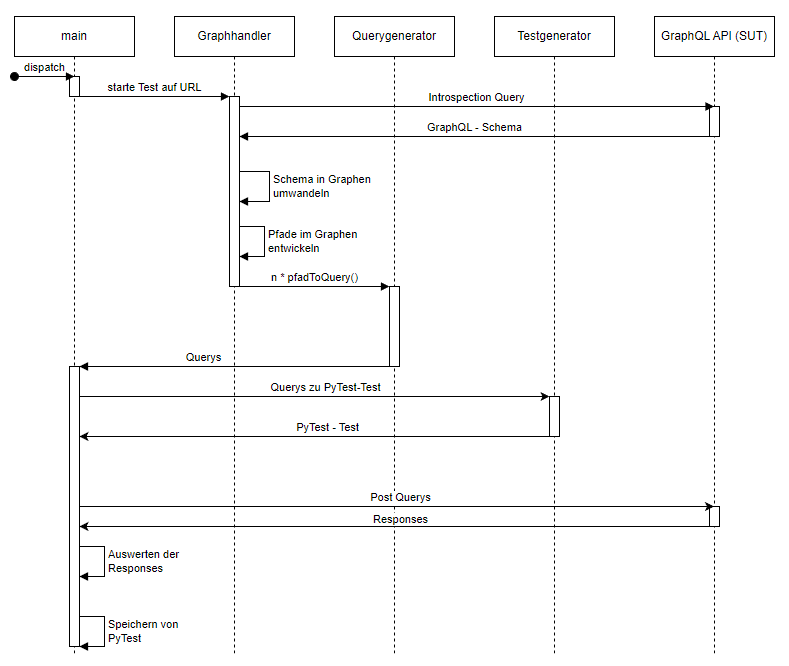
\includegraphics[width=\textwidth,height=\textheight,keepaspectratio]{img/sequenz}
    \end{center}
    \caption{Sequenzdiagramm des Prototypens}
    \label{sqzd}
\end{figure}

Hierbei sind auch die einzelnen Module zu erkennen.
Dabei sind die Module $main$, $Graphhandler$, $Querygenerator$ und $Testgenerator$ Teile des Prototypens.
Das Modul $GraphQL API$ stellt das zu testende System dar und ist extern.
Die Module $Graphhandler$, $Querygenerator$ und $Testgenerator$ arbeiten chronologisch.
Hierbei übernimmt der $Graphhandler$ alle Teile des Testentwurfs also alle Teile des Kapitels~\ref{testentw}.
Der $Querygenerator$ übernimmt die Umsetzung der Methode aus Kapitel~\ref{testentw}.
Im $Testgenerator$ werden die PyTest-Tests generiert, dies ist ein gewünschtes Feature aus Kapitel~\ref{testf}.
Die $main$ verwaltet die Zusammenarbeit der einzelnen Module und sorgt für die Umsetzung aller übrigen Funktionen.

\subsection{Schema in Graph abbilden}

Wie in der Vorstellung der Methode im Kapitel~\ref{schemagraph} erwähnt, muss das GraphQL-Schema in einem Graphen abgebildet werden.
Der Graph wird in einem gerichteten NetworkX-Graphen abgebildet.
In einem ersten Schritt wird jedoch die Introspection-Query~\ref{introspection-query} ausgeführt, um Informationen über das Schema des SUT zu erlangen.
Es sei angemerkt, dass einige GraphQL APIs so eine Introspection-Query verbieten, sei es einerseits durch direktes Unterbinden oder ein Tiefenlimit in den Querys.
Das SUT muss in jedem Fall die Introsepction-Query unterstützen, da sonst keine Informationen über das GraphQL-Schema erlangt werden können.
Die Query wird mit einem simplen HTTP-POST an die zu testende URL gesendet.

\begin{lstlisting}[language=Python, caption={Absenden der Introspection-Query}]
r = requests.post(testUrl, json={'query': queries.introspection_query})
json_data = json.loads(r.text)
\end{lstlisting}

Die Response erfolgt als JSON-Objekt.
Erhaltene Daten werden in der Variable $json\_data$ gespeichert.
Im $Graphhandler$ Modul wird dann mit der Funktion $buildGraph$ ein gerichteter NetworkX-Graph aus dem GraphQL-Schema erstellt.
Diese generiert rekursiv einen Graphen von einem gegebenen Startknoten, einem leeren Graphen und dem Schema.
Es werden nur erreichbare Knoten vom Startknoten berücksichtigt.
Wird der Startknoten auf den Knoten $Query$ gesetzt, so wird jeder erreichbare Teil des Graphens hinzugefügt, der vom $Query$ Knoten erreichbar ist.
Dies ist insofern sinnvoll, als andere Typen, wenn sie nicht von $Query$ aus erreichbar sind, nicht Teil des Testraumes wären, da diese in keiner validen Anfrage vorkommen können.
Die Funktion, die den Graphen generiert, ist in Abbildung~\ref{graphbuild} dargestellt.

\begin{figure}
    \begin{lstlisting}[language=Python]
def buildGraph(graph, type_name, type_dict):
    if type_name.startswith(nonSchemaTypePrefix) or type_name in baseDatatypes:
        pass
    else:
        for adjacentNode in type_dict[type_name]['fields']:
            if graph.has_edge(type_name, adjacentNode['type']['name']):
                return
            else:
                if adjacentNode['type']['name'] and adjacentNode['type']['name'] not in baseDatatypes:
                    graph.add_edge(type_name, adjacentNode['type']['name'])
                    graph[type_name][adjacentNode['type']['name']]["data"] = adjacentNode
                    buildGraph(graph, adjacentNode['type']['name'], type_dict)
                if adjacentNode['type']['kind'] == 'LIST' and adjacentNode['type']['ofType']['name'] not in baseDatatypes:
                    graph.add_edge(type_name, adjacentNode['type']['ofType']['name'])
                    graph[type_name][adjacentNode['type']['ofType']['name']]["data"] = adjacentNode
                    buildGraph(graph, adjacentNode['type']['ofType']['name'], type_dict)
    \end{lstlisting}
    \caption{Funktion die einen gerichteten Graphen aufspannt}
    \label{graphbuild}
\end{figure}

Die Funktion buildGraph arbeitet rekursiv.
Vom Startknoten aus ruft die Funktion alle Folgeknoten von Query auf.
Dies sind alle Knoten, die den Type $OBJECT$ besitzen und nicht mit einem $\_\_$ beginnen oder ein Basisdatentyp sind.
GraphQL kann eigene Objekte definieren, welche mit $\_\_$ starten.
Diese werden explizit ausgeschlossen, genau wie alle $SCALAR$ Types.
Jeder Knoten definiert in seinem $fields$ Eintrag, zu welchen Feldern er Beziehungen hat.
Hierbei muss unterschieden werden, dass ein Eintrag entweder vom Type $OBJECT$, $NON\_NULL$ oder $LIST$ sein kann, um zulässig zu sein.
Sollte es sich um einen $LIST$ oder $NON\_NULL$ Eintrag handeln, muss geprüft werden, von welchem Type diese sind.
Wenn ein Knoten alle Bedingungen erfüllt, so wird dieser dem Graphen hinzugefügt und auf ihm selbst wird $buildGraph$ ausgeführt.
So wird der gesamte Graph rekursiv aufgebaut und jeder erreichbare Knoten vom Startknoten wird einbezogen.

\newpage
\subsection{Pfade aus Graph bilden}

Der Graphhandler implementiert verschiedene Abdeckungskriterien.
Das Tool benötigt im Verlauf eine Liste $paths$ aller Pfade, die für die Testgenerierung berücksichtigt werden sollen.

\begin{figure}[H]
    \begin{lstlisting}[language=Python]
paths = graphhandler.generate_prime_paths("Query", graph)
    \end{lstlisting}
    \caption{$paths$ als Liste von Pfaden für ein Abdeckungskriterium}
\end{figure}

Wie im Kapitel~\ref{fazitcov} festgestellt, gilt, dass die PrimePfad-Abdeckung am geeignetsten ist und somit wird diese implementiert.
Die PrimePfad Abdeckung ist durch die Funktion $generate\_prime\_paths$ implementiert.
Diese Funktion verknüpft dabei zwei andere Funktionen und ist in Listing~\ref{primes} gezeigt.

\begin{lstlisting}[language=Python,caption={valide PrimePfad Generierung}, label={primes}]
def generate_prime_paths(startknoten, g):
    return shortest_path_to_prime(g, startknoten, get_prime_paths(g, startknoten))
\end{lstlisting}

Da PrimePfade nicht im Query Knoten starten müssen, wird zuerst die Funktion $get\_prime\_paths$ aufgerufen.
Diese gibt eine Liste aller PrimePfade zurück.
Da jedoch ein Testpfad stets im Query-Knoten starten muss, wird anschließend $shortest\_path\_to\_prime$ ausgeführt.
Diese Funktion ermittelt den kürzesten Weg vom Query-Knoten zum Startknoten des PrimePfades.
So kann sichergestellt werden, dass die generierten PrimePfade stets korrekte Testpfade sind.
Die Implementierung der Funktion $get\_prime\_paths$ ist im Listing~\ref{primepy} gezeigt.

\begin{lstlisting}[language=Python, caption={PrimePfad Algorithmus}, label={primepy}]
def get_prime_paths(G, start_node):
    startPaths = [(n, ) for n in g.nodes()]
    simplePaths = []
    findSimplePath(g, startPaths, simplePaths)
    primePaths = sorted(simplePaths, key=lambda a: (len(a), a))
    return primePaths
\end{lstlisting}

Von jedem Knoten ausgehend werden die einfachen Pfade ermittelt.
Anschließend werden die Pfade so gefiltert, dass nur die längsten Pfade, die kein Teilpfad eines anderen Pfads sind, zurückgegeben werden.
Dies entspricht laut Definition~\ref{primepfad} einem PrimePfad und der Algorithmus ist Deckungsgleich mit~\cite[Finding Prime Test Paths S. 39]{software-testing}.
Für Pfade die keinen Ursprung im Query-Knoten haben wird der kürzeste Weg vom Queryknoten zum Startknoten des Pfades ermittelt.
So wird die Korrektheit der Testpfade sichergestellt.

\newpage
\subsection{Querys aus Pfad ermitteln}

Aus den entwickelten Pfaden sollen Querys entwickelt werden, sodass diese an die GraphQL-API gestellt werden können.
Eine Query beginnt in GraphQL immer im Query-Knoten und so beginnt jeder Pfad in diesem Knoten.
Um die Wahrscheinlichkeit zu erhöhen, dass ein Pfad gut abgedeckt wird, werden pro Pfad mehrere Querys entwickelt.
Hierfür wurde die Variable $testPerPath$ angelegt, diese legt fest, wieviele Querys pro Pfad generiert werden sollen.
Standardmäßig gilt: $testPerPath = 5$.
Die Generierung der Querys übernimmt die Methode $pathToQuery$ vom Modul $Querygenerator$.
In der Methode $pathToQuery$ wird ein Pfad mithilfe eines Typedict und dem Graphen zu einer validen GraphQL-Query umgewandelt.
Die Funktion $pathToQuery$ entfernt den Startknoten Query und reichert den Pfad an.
Ihre Implementierung ist in Listing~\ref{querp} dargestellt.

\begin{lstlisting}[language=Python, caption={Funktion pathToQuery}, label={querp}]
def pathToQuery(path, typedict, graph):
    path_edges = list(zip(path[:-1], path[1:]))
    query = "{ " + resolvePathTillOnlyScalarTypesOrEnd(path_edges, typedict, graph) + " }"
    return query
\end{lstlisting}

Die Funktion erstellt eine Query, indem der angegebene Pfad abgelaufen wird und mit Argumenten angereichert, falls nötig.
Das Ablaufen des Pfads und die Anreichung mit Argumenten übernimmt die rekursive Funktion \\
$resolvePathTillOnlyScalarTypesOrEnd(path, typedict, graph, query="")$ die in Listing~\ref{respath} dargestellt ist.

\begin{lstlisting}[language=Python,caption={Pfadumwandlung in Query}, label={respath}]
def resolvePathTillOnlyScalarTypesOrEnd(path, typedict, graph, query=""):
    if path:
        edge = path.pop(0)
    else:
        return query
    edge_data = graph[edge[0]][edge[1]]["data"]
    if len(edge_data['args']) < 1:
        if edge_data["type"]["kind"] == "SCALAR":
            query = query + " " + edge_data["name"] + " "
        else:
            query = query + " " + edge_data["name"] + " { " + addScalarTypes(edge_data["type"], typedict, edge_data["name"]) + " " + resolvePathTillOnlyScalarTypesOrEnd(path, typedict, graph, query) + " } "
    else:
        argString = edge_data['name'] + "("
        for args in edge_data['args']:
            argString = argString + args["name"] + ": " + resolveArg(args["type"], typedict) + ", "
        argString = argString + ")"
        query = query + argString + " { " + addScalarTypes(edge_data["type"], typedict, edge_data["name"]) + " " + resolvePathTillOnlyScalarTypesOrEnd(path, typedict, graph, query) + " } "
    return query
\end{lstlisting}

Die Funktion fügt für jeden Knoten alle definierten $SCALAR$ Felder hinzu.
So wird sichergestellt, dass alle einfachen Felder eines Objektes abgefragt werden.
Es wird so validiert, dass das Objekt übereinstimmt mit der Schema-Definition.
Sind alle $SCALAR$ Types hinzugefügt, so wird geprüft, welches Feld vom Type $OBJECT$ hinzugefügt werden muss, um die Kante zum nächsten Knoten abzubilden.
Sollte diese Kante Einträge im $args$ Feld besitzen, so werden passende Argumente generiert.
Da Argumente nur $SCALAR$ Types oder Aggregationen von $SCALAR$ Types sein können, werden Datengeneratoren für die Standarddatentypen benötigt.
Die Zuweisung der Datengeneratoren geschieht hierbei mit der Funktion $resolveArg$.
Benötigt ein $OBJECT$ Feld Argumente, so werden diese der Query hinzugefügt, indem mit $resolveArg$ die Argumente zur Verfügung gestellt werden.
Anschließend wird die Kante aus der Liste des Pfads entfernt und die Funktion wieder rekursiv aufgerufen.
Abbruchbedingung ist, dass der Pfad keine Kanten mehr besitzt.
Wenn der Pfad keine Kanten mehr besitzt, so ist die entwickelte Query ein Test, der den Pfad abdeckt.
Es sei angemerkt, dass durch die zufällige Argumentgenerierung keinesfalls garantiert ist, dass bei der Testausführung der volle Pfad getestet wird.
Sollte zum Beispiel ein Pfad direkt am Anfang Argumente benötigen, diese aber jedoch zu keinen Daten des SUT passen, so ist es wahrscheinlich,
dass der Test erfolgreich sein wird, ohne dass der eben entwickelte Pfad wirklich komplett getestet wird.
\newpage

\subsection{Tests ausführen \& Testdatei generieren}

Bevor die Tests ausgeführt werden, sind diese im PyTest-Format zu speichern.
Dafür wird eine Datei angelegt, die alle nötigen Imports enthält.
Anschließend wird für jede Query ein eigener Test angelegt und die Auswertung festgeschrieben.
Implementiert wurde dies in der Funktion $generatTestFromQuery$ im Modul $Testgenerator$.
Ein so erstellter PyTest ist in Listing~\ref{pytestt} dargestellt.

\begin{lstlisting}[language=Python, caption={PyTest einer Query}, label={pytestt}]
def testQuery6aa8b26(caplog):
    caplog.set_level(logging.WARNING)
    response = requests.post(testUrl,json={'query':"{...}")
    response_as_dict = json.loads(response.text)
    measurement = queries.compareQueryResults(response_as_dict, "{...}")
    if measurement["expectedPathLength"] > measurement["pathLengthFromResult"]:
        logging.warning(" Test hat nicht 100% Abdeckung ")
    assert response.status_code == 200
\end{lstlisting}

Nachdem mit den PyTests die Querys reproduzierbar gemacht wurden, werden die Querys ausgeführt.
Hierbei setzt der Code aus Listing~ref{testt} die Ausführung um.


Hierbei wird der Code aus Listing~\ref{testt} genutzt.
Eine Query wird als HTTP-POST an das SUT gestellt, die Antwort wird dann auf ihre Pfadlängen hin untersucht und in
einer Datei abgespeichert.

\begin{lstlisting}[language=Python, caption={Ausführen einer Testquery}, label={testt}]
queryResults = []
for testQuery in primePathQueries:
    r = requests.post(testUrl, json={'query': testQuery}, headers=HEADERS)
    response_as_dict = json.loads(r.text)
    measurement = queries.compareQueryResults(response_as_dict, testQuery)
    queryResults.append([testQuery, r, measurement])
    f.write(" => ".join([testQuery, r.text]))
    f.write("\n")
f.close()
\end{lstlisting}

Um die Tests auszuführen, werden alle generierten Querys an das SUT gesendet.
Die Antworten werden bemessen, gespeichert und später ausgewertet.

\subsection{Testauswertung}

Die Testauswertung erfolgt, wie zuvor gesehen, auf zweierlei Arten.
Einerseits werden Tests ad-hoc ausgeführt.
Andererseits wird eine Datei mit PyTests generiert.
Die Auswertung der Testquerys in der PyTest-Datei erfolgt nach PyTest-Standard. Dabei werden Hinweise geliefert, wenn etwas von der Erwartung abweicht.
Eine Auswertung der Testquerys, die direkt ausgeführt wurden, erfolgt nach einer Kategorisierung.
Die Kategoriesierungen sind \textbf{Good\_Test},\textbf{Perfect\_Test},\textbf{malformed\_Test} und \textbf{confirmed\_failed\_Test}.
Ein \textbf{Good\_Test} ist ein Test, der keinen Fehler erzeugt hat.
Dieser hat allerdings auch nicht die erwartete Pfadlänge von der Response erfüllt, es war also ein Test,
der nicht die komplett gewünschte Abdeckung erreicht hat.
\textbf{Perfect\_Test} sind Tests, die keinen Fehler erzeugt haben und die erwartete Pfadlänge entspricht der Pfadlänge der Response.
Eine solche Query hat den Pfad, der zu testen war, ideal abgedeckt.
\textbf{malformed\_Test} sind Tests, die fehlerhaft sind, aber allerdings aufgrund von Generierungsfehlern des Prototypen.
\textbf{confirmed\_failed\_Test} sind Tests, bei denen tatsächlich einen Fehler gefunden wurde.
Die fehlerhaften Tests werden dann im Folgenden ausgegeben mit der konkreten Fehlerbeschreibung, sodass eine Fehleranalyse möglich wird.
Um Maß darüber zu halten, wie viele Tests in welcher Kategorie sind, wurde eine Auswertung geschrieben, welche in Listing~\ref{auswert} gezeigt ist.

\begin{lstlisting}[language=Python, caption={Auswertung der Antworten}, label={auswert}]
successfull = 0
perfect = 0
own_failure = 0
server_failures = 0
testCount = 0

for queryResult in queryResults:
    testCount = testCount + 1
    if any(substring in queryResult[1].text for substring in ["GRAPHQL_PARSE_FAILED", "GRAPHQL_VALIDATION_FAILED"]):
        own_failure = own_failure + 1
    elif "INTERNAL_SERVER_ERROR" in queryResult[1].text or r.StatusCode == 500:
        server_failures = server_failures + 1
    elif "data" in queryResult[1].text and queryResult[2]["expectedPathLength"] > queryResult[2]["pathLengthFromResult"]:
        successfull = successfull + 1
    elif "data" in queryResult[1].text and queryResult[2]["expectedPathLength"] == queryResult[2]["pathLengthFromResult"]:
        perfect = perfect + 1
\end{lstlisting}

\newpage

\section{Zusammenfassung der Implementation}

Der Python Prototyp stellt eine Implementierung der Methode aus Kapitel~\ref{testentwurf} dar.
Wie später gezeigt wird, ist der Prototyp in der Lage, reale Fehler in GraphQL-APIs zu finden.
Die modulare Aufbauweise des Prototypens erlaubt es, dass zukünftige Anpassungen an der Software einfach umsetzbar sind.
So sind die Module thematisch getrennt und das Anpassen sowie Auswechseln einzelner Module ist möglich, ohne die Funktionsweise
der anderen Module zu beeinträchtigen.


